\documentclass[11pt]{article}% uses letterpaper by default

%---------- Uncomment one of them ------------------------------
\usepackage[includeheadfoot, top=0.5in, bottom=0.5in, hmargin=1in]{geometry}

\usepackage{fancyhdr}
\usepackage{setspace}
\renewcommand{\footrulewidth}{0.4pt}% default is 0pt
\pagestyle{fancy}
\usepackage{graphicx}
\singlespacing
\usepackage{amsmath}
\usepackage{url}
\usepackage{hyperref} 
\usepackage{xcolor}
\hypersetup{ 
     colorlinks=true, 
     linkcolor=blue, 
     filecolor=blue, 
     citecolor=black,       
     urlcolor=cyan} 
% urlcolor = URL links, linkcolor = within-PDF links

% \newcommand*{\mt}{\mathrm}
% \newcommand*{\unit}[1]{\;\mathrm{#1}}  % vemod.net/typesetting-units-in-latex
% \newcommand*{\abt}{\mathord{\sim}} % tex.stackexchange.com/q/55701
% \newcommand*{\Msun}{\mathrm{M}_{\sun}}

\newcommand{\SPACE}{\vspace{3em}}
\newcommand{\degrees}{\ensuremath{^\circ}}
\newcommand{\arcmin}{\ensuremath{'}}
\newcommand{\arcsec}{\ensuremath{"}}
\newcommand{\hours}{\ensuremath{^\mathrm{h}}}
\newcommand{\minutes}{\ensuremath{^\mathrm{m}}}
\newcommand{\seconds}{\ensuremath{^\mathrm{s}}}
\newcommand{\labnumber}{06}  % UPDATE THIS!

\usepackage{datetime2}  % customize \today, defaults to yyyy-mm-dd
\lhead{ASTR UN1903 -- Lab \labnumber}
\lfoot{M. Sayeed}
\cfoot{\thepage}
\rfoot{\today}
\rhead{Mondays 6-9 pm}
\renewcommand{\rightmark}{}
\renewcommand{\headrulewidth}{0pt}
\renewcommand{\footrulewidth}{0.4pt}
% -----------------------------
% End personal config (AT, Sp 2019)
% -----------------------------

\newcommand*{\mt}{\mathrm}
\newcommand*{\unit}[1]{\;\mathrm{#1}}  % vemod.net/typesetting-units-in-latex
\newcommand*{\Msun}{\mathrm{M}_{\sun}}

% Compact spacing
\setlength\parindent{0pt}
\setlength{\parskip}{1em}

% -----------------------------
% End personal config (AT, Sp 2019)
% -----------------------------


\begin{document}

\begin{center}
\Large\textbf{Lab \labnumber: The Sun Lab}
\end{center}

\section{Light}

Light acts like both a wave and a particle, as you may have heard.

\textbf{Waves} are traveling vibrations in space and time.
\begin{itemize}
\item Freeze a wave in time: you can measure a wavelength ($\lambda$, Greek
    letter lambda) from peak to peak or trough to trough
\item Stand next to a wave: you can time how long it takes for consecutive
    peaks or troughs to pass by, thus you can measure a period ($T$) or
    frequency ($f = 1/T$).
\end{itemize}
The frequency, wavelength, and speed $c$ of a wave are related as:
\[
    c = f \lambda
\]
A \textbf{photon}, which is a particle (or quantum) of light, has energy
\[
    E = h f
\]
where $h$ is Planck's constant and $f$ is frequency.

Light has a \textbf{spectrum}, which is its intensity as a function of
wavelength, $I(\lambda)$.
To figure out how bright an object appears to the human eye, you would add up
all the light between $400$ and $700 \unit{nm}$ as
\[
    \int_{400\unit{nm}}^{700\unit{nm}} I(\lambda) \mathrm{d}\lambda .
\]
You may see different definitions for ``spectrum''; e.g., \{intensity, flux,
specific flux, specific intensity, brightness, irradiance\} as a function of
\{wavelength, frequency, energy\}.
All mean roughly the same thing for this class.

Lastly, matter can \textbf{emit}, \textbf{reflect}, \textbf{absorb}, and
\textbf{transmit} light.

\begin{enumerate}
    \item The speed of light, $c$, is constant. What does that imply about the
    relationship between $f$ and $\lambda$?\SPACE
    \item Which form of light has higher frequency: X-rays or infrared?\SPACE
    \item Which form of light has more energy: microwave or visible?\SPACE
    % instructor note: draw the EM spectrum on the board in terms of __wavelength__ (BUT don't draw any other axes, let students deduce)
    \item If you shine white light (all visible wavelengths) upon a Red Delicious
    apple, it absorbs blue and green light but reflects red. Thus we perceive the
    apple as red.
    \begin{enumerate}
        \item What wavelengths of visible light does a snowball reflect? Absorb?\SPACE
        \item Why do black objects heat more in sunlight than white objects?\SPACE
        \item What happens if you shine a blue light on a red apple? What about a red light?\SPACE
    \end{enumerate}
\end{enumerate}

All objects emit light.  That light has a \textbf{blackbody} spectrum,
dependent only on the emitting object's temperature.
\begin{center}
    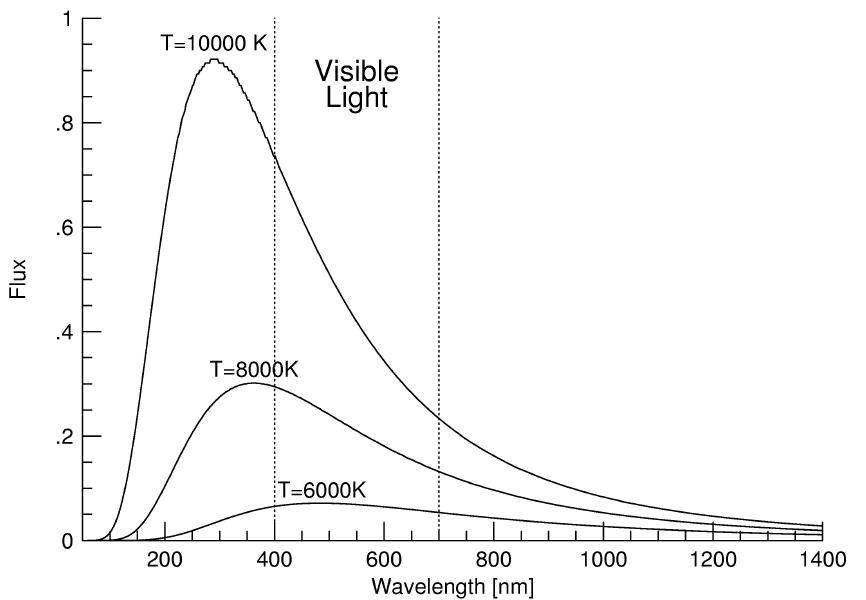
\includegraphics[width=0.6\textwidth]{bb3T.jpg} \\
    \small{Credit: \href{http://www.astronomy.ohio-state.edu/~thompson/161/spectra.html}{R.~Pogge, T.~Thompson (OSU)}}
\end{center}
Hotter things emit more brightly and emit more at small wavelengths (so, they
look bluer to the eye).
The wavelength where a blackbody emits most strongly is given by:
\[
    \lambda_\mathrm{max} = \frac{0.29 \unit{cm\;K}}{T}
\]
where $T$ has units of Kelvin.

\begin{enumerate}
    \item What would a hot star ($T=10,000\unit{K}$) look like to your eye? What is its $\lambda_\mathrm{max}$?\SPACE
    \item What would a cool star ($T=3500\unit{K}$) look like to your eye?  What is its $\lambda_\mathrm{max}$?\SPACE
    \item The hot star emits more red light than the cool star. But, the hot star looks blue and the cool star looks red. Why is this? Explain in your own words. {\small You can check by looking at two very bright winter-sky stars, Sirius (hot) and Betelgeuse (cool), with your naked eye -- which hopefully we'll do later this term!}\SPACE
\end{enumerate}

Finally, here are a few plots of the Sun's spectrum.
%Note the differing $x$- and $y$-axis scales.
\begin{center}
    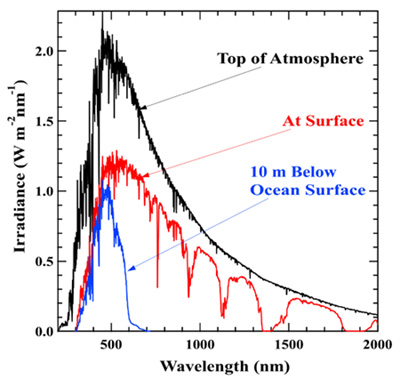
\includegraphics[width=0.45\textwidth]{SolarSpectrum2.jpg} \\
\end{center}
{\small
Solar spectrum above Earth's atmosphere, i.e., space (black), at Earth's surface
(red), and underwater (blue).
Credit: \href{http://lasp.colorado.edu/~bagenal/3720/CLASS4/4Sunlight.html}{F.~Bagenal (CU Boulder)}
}
\begin{center}
    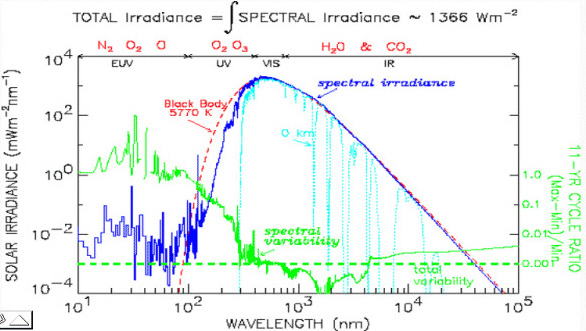
\includegraphics[width=0.85\textwidth]{solar_spectrum_loglog.jpg} \\
\end{center}
{\small
Solar spectrum from space (dark blue), at Earth's surface (cyan), and model
blackbody spectrum for Sun's surface temperature (dashed red).
Spectral variability (light green, right $y$-axis) shows
how much the Sun 's spectrum varies over a solar cycle.
The Sun 's UV and EUV intensity can change by up to $2\times$, whereas the
sun's visible intensity only varies by 0.1\%.
Credit: \href{http://www.physics.unlv.edu/~jeffery/astro/sun/solar_spectrum_graph_2.html}{NRL/NASA, posted by D.~Jeffery (UNLV)}
}

The dips in the spectrum are \textbf{absorption lines}.
Atoms in both the Sun's atmosphere and Earth's atmosphere absorb light at very
specific frequencies, causing us to miss some blackbody spectrum light that
would have otherwise reached us.

\section{The Sun}\label{sec:vid}

We'll watch a series of videos
(\url{http://www.pbs.org/wgbh/nova/labs/videos/\#sun}) introducing solar
science and the Helioviewer.

For Sections~\ref{sec:vid} your answers can be brief; a
few words or a sentence will do.

\begin{enumerate}
%\item How long does it take a photon to travel from the core of the Sun , where it's produced, to the surface?
%\item Describe the 3 forces that are most relevant in the Sun .
%\item Do your best to draw the magnetic field lines around the Sun in your lab notebook.
\item What causes the Sun's magnetic field to become both stronger and more
    tangled?\SPACE
\item How long does it take the Sun to rotate once on its own axis?\SPACE
\item Name two events that can be caused by magnetic reconnection.\SPACE
\item Define ``solar maximum''.\SPACE
\item Why do sunspots look darker than the rest of the Sun ?\SPACE
\item What are two ways that Earth is protected from solar storms?\SPACE
\item What causes auroras?\SPACE
\item Why are humans more vulnerable to big solar storms now than in 1859?\SPACE
\item Is the following statement true or false? ``The longer its wavelength, the more energy light carries.'' Explain why.\SPACE
\item Why is it useful for solar research to have instruments that can look at wavelengths besides the visible that we can see with our eyes?\SPACE
\item If you want to look at a hotter part of the solar atmosphere, do you want to look at smaller or larger wavelength light?\SPACE
\item What is special about the STEREO mission?\SPACE
\item Describe the instruments on the SDO (AIA, HMI).\SPACE
\end{enumerate}

% \section{Solar Cycle}\label{sec:cycle}

% Click the Solar Cycle tab on this page and follow the instructions while
% answering the following questions:
% \url{http://www.pbs.org/wgbh/nova/labs/lab/sun/research}
% \begin{enumerate}
% \item Record your estimates of R and the scientific estimates as you go.\SPACE
% \item How do your estimates of R compare to the scientific estimates?  If your estimate differed, why do you think that was so?\SPACE
% \item After completing your five estimates, how do your measurements (orange highlighted points) compare to the official solar cycle measurements?\SPACE
% \end{enumerate}


% \section{Storm Prediction}\label{sec:storm-pred}

% Click the Storm Prediction tab on this page and follow the instructions
% while answering the following questions:
% \url{http://www.pbs.org/wgbh/nova/labs/lab/sun/research}
% \begin{enumerate}
% \item Record your answers, and how you did compared to the correct answers.\SPACE
% \item Which of these was hardest for you to decide?  Easiest?\SPACE
% %\item What does the size of a sunspot tell us about the Sun's magnetic field and how does it help us predict solar storms?
% %\item What does the complexity of sunspots tell us?
% %\item What does rapid sunspot growth tell us about the Sun's magnetic field?
% %\item How does the mixing of magnetic fields help us to predict solar flares or CMEs?
% %\item While observing the chromosphere and corona of the Sun, scientists often
% %observe bands of plasma, called filaments. What can these filaments tell us
% %about the possibility of a solar storm?
% \end{enumerate}

\section{Forming Questions}

Hop onto Helioviewer: \url{http://helioviewer.org/}
Your TA will walk through the features.  Play around for a bit.
Several resources -- including a guide to SDO/AIA images -- are linked towards
the end of this lab.

Now, you will generate some research questions about the Sun.
What does that mean?  That often (but not always) means investigating
cause-and-effect, e.g. by looking for correlation.

For example, one may ask: what features in the Sun develop before a flare?
Suppose you do find something at $171$ \AA just before one flare.
That can lead to a host of follow-up questions:
is more stuff happening at other wavelengths, before this flare?
Can you relate the feature to the flare properties and aftermath?
Are the same features seen for other flares?  If not, why?

Ask many questions, and strive to form \emph{testable} questions and
\emph{falsifiable} hypotheses.  Explore the data as you go -- you will probably
answer some of your simpler questions just by looking at the data, and gain
ideas for new questions.
I recommend recording all questions/ideas you've considered, even those that
you discard; you might later realize that a seemingly-intractable question is
quite doable!
\newpage
\begin{enumerate}
\item Record at least 3 research questions, and explain how you would investigate these questions using the available data. Please come up with questions \textbf{individually} even if you are working in a group; everyone's questions in your group should be different, but feel free to discuss ideas with other students.\SPACE \SPACE
\end{enumerate}

% \begin{center}
%     
\includegraphics[width=0.6\textwidth]{magical_world_crop.png} \\
%     \small{C\&H, Bill Watterson, 1995 Dec 31}
% \end{center}

\section{Investigation}

Find a partner and choose a research question to investigate in depth. \textbf{Run your question by the TA before you begin.} As you study the data, your question may change slightly, or you may even wish to throw it out entirely.  That's OK and encouraged!  But, please explain in your write-up how/why you changed course.

\textbf{Write-up expectations}

Your lab write-up should make very clear:
\begin{enumerate}
\item What is the question you are investigating?\SPACE
\item What is your plan to answer this question?\SPACE
\item How did you execute the plan, how did it go?\SPACE
\item Explain the conclusion you came to, and how the data support this conclusion.\SPACE
\end{enumerate}

You will be graded on demonstrated effort, scientific thinking, and clarity of
presentation.
Your conclusions should be supported by the Helioviewer data, but you will not
be penalized for slightly incorrect conclusions due to insufficient time/data.
Pretend you are a scientist writing a rough draft of a scientific paper
(which you are!).
Write down your thinking as you go along.
Do use complete sentences or coherent sentence fragments.

Don't assume that your TA can see what you see.
Think about what you will highlight, and be quantitative when necessary.
Regarding an appropriate level of detail, here are two example statements that
describe the same feature:
\begin{itemize}
\item ``...filament A (x=963", y=165" at 2020/02/02 02:02:02UT) is twice the
    diameter of its underlying sunspot group (IX) and persists for the sunspot
    group's entire journey from left to right limb of the Sun; filament A
    seems to vibrate with respect to group IX when we toggle images with 1 hr
    spacing, but we saw no vibration when toggling with 10 minute or 1 minute
    spacing, though this could have been due to image noise or limited human
    eye sensitivity...''
\item ``...we saw a big, dark bar over one sunspot group, and decided to look for more examples; we found 20 similar bars in Feb 01--28, 2020...''
\end{itemize}
Each statement communicates very different information. Neither one nor other is ``better''; ``better'' depends on context.  But, if you are unsure, err on the side of more detail.

\section{Conclusions}
\begin{enumerate}
    \item What did you like or dislike about this lab?  \SPACE
    \item Any feedback/suggestions?\SPACE
    \item Any remaining questions?\SPACE
\end{enumerate}

% \textbf{Presentation}: see first page of lab.  If everyone is done
% investigating/writing by 9:30pm on March 06, and no one is waiting for movies
% to render, we can do the presentations right away and conclude the lab sequence
% early.

%at the start of the March 13 lab you will present your results to the rest of
%the class. Your presentation should be less than 5 minutes and should include
%\begin{itemize}
%\item your question
%\item your conclusion / other outcome of your investigation
%\item 1--2 images or movies from Helioviewer to support your conclusion
%\end{itemize}

\newpage
\pagebreak
\appendix

\section{About the Sun}

\begin{itemize}
    \item Solar cycle: 11 years
    \item Sunspot counts, 2008-2019: \\
        \url{https://www.swpc.noaa.gov/products/solar-cycle-progression}
    \item Sun's rotation period: 24.5 days (equator), 38 days (poles) \\
        Sun's rotation period, synodic (equator): 26.24 days \\
        Sun's rotation period, synodic (lat=26 deg): 27.2753 days, called the Carrington period
\end{itemize}

\section{Data catalogs and archives}

A few examples, sorted in rough descending order of (anticipated) usefulness.
Google around to find more!

\begin{itemize}
    \item SOHO/LASCO coronal mass ejections \url{https://cdaw.gsfc.nasa.gov/CME_list/}
        manually identified by humans
        \begin{itemize}
        \item Example:
            \href{https://cdaw.gsfc.nasa.gov/CME_list/UNIVERSAL/2011_05/jsmovies/2011_05/20110509.205726.p073g/c2_rdif.html}{movie of strong CME, 2011/05/09 20:57:26UT}
        \item Example:
            \href{https://cdaw.gsfc.nasa.gov/CME_list/UNIVERSAL/2012_07/jsmovies/2012_07/20120723.023605.p286g/c2_rdif.html}{movie of strong CME, 2012/07/23 02:36:05UT}
        \item Note that one CME is accompanied by a burst of X-rays, but the
            other is not.  Why??
        \end{itemize}
    \item Hinode/XRT-detected X-ray flares (2006-2017) \url{http://xrt.cfa.harvard.edu/flare_catalog/all.html}
    \item RHESSI-detected X-ray flares (2002-2018) \url{http://hesperia.gsfc.nasa.gov/hessidata/dbase/hessi_flare_list.txt}
        with start and end times, peak X-ray photons per second (``P c/s'',
        peak counts/second), total counts, flare's position on the Sun .
        Warning, text file size is 17MB.
    \item ACE solar wind measurements (1998-2018)
        \url{http://www.srl.caltech.edu/ACE/ASC/DATA/level3/summaries.html}
        including wind velocity, particle density, magnetic field, etc.
        sensed at a location between Earth and Sun (quite close to Earth, at L1
        Lagrange point).
        You can ask, for example, what features on the Sun correlated with high
        levels of carbon ions hurling towards Earth?
\end{itemize}

\section{Helioviewer help!}

\begin{itemize}
    \item The ``measurement'' values are the wavelength, in Angstroms
        (\AA), of the filter used to obtain the image.
        $1 \unit{\AA} = 10^{-10} \unit{m} = 10 \unit{nm}$.
    \item If the date/time turns red or yellow, that means there is not data of
        the requested type taken close to the date/time you asked for.  Even if
        the date/time is green, it's best to check to see what time is actually
        being displayed, as opposed what time you input.
    \item Helioviewer User guide: \\
        \url{http://wiki.helioviewer.org/wiki/Helioviewer.org_User_Guide_3.1.0}
    \item Helioviewer ``Features and Events'' annotations on Helioviewer: \\
        \url{http://wiki.helioviewer.org/wiki/HEK_Features_and_Events}
    \item Glossary of solar physics terms: \\
        \url{https://hesperia.gsfc.nasa.gov/sftheory/glossary.htm}
    \item What do SDO images show? \\
        \url{https://www.nasa.gov/mission_pages/sunearth/news/light-wavelengths.html}
    \item What do SDO images show? (same image, slightly more detailed explanation) \\
        \url{https://www.nasa.gov/content/goddard/how-sdo-sees-the-sun}
\end{itemize}

\section{Cheat-sheet of Helioviewer data}

\begin{itemize}
\item SDO: 2010 to present
    \begin{itemize}
    \item Cadence: ~30 seconds (for same wavelength image)
    \item AIA: 94, 131, 171, 193, 211, 304, 335, 1600, 1700, 4500 \AA
    \item HMI: continuum, magnetogram
    \end{itemize}
\item SOHO: 1995 to present
    \begin{itemize}
    \item Cadence: 12 minute (?)
    \item EIT: 171, 195, 284, 304 \AA
    \item LASCO: C2 (inner), C3 (outer) white-light coronagraph
    \item MDI: continuum, magnetogram
    \end{itemize}
\item STEREO-A: 2007 to present
\item STEREO-B: 2007 to 2014
    \begin{itemize}
    \item Positions: \url{https://stereo-ssc.nascom.nasa.gov/cgi-bin/make\_where\_gif}
    \item Cadence: 3 minute (?at best)
    \item SECCHI EUVI 171, 195, 284, 304 \AA
    \item SECCHI COR1 white-light coronagraph (inner)
    \item SECCHI COR2 white-light coronagraph (outer)
    \end{itemize}
\item TRACE: 1998 to 2010
    \begin{itemize}
    \item 171 \AA (ionized Fe), 195  \AA (ionized Fe), 284 \AA (ionized Fe),
        1216 \AA (neutral H), 1550 \AA (ionized C), 1600  \AA (continuum),
        1700 \AA (continuum)
    %171 (FeIX), 195 (FeXII), 284 (FeXV), 1216 (HI), 1550 (CIV)
    \end{itemize}
\item Yohkoh: 1991 to 2001
    \begin{itemize}
    \item Soft X-ray telescope
    \item Some movies at \url{http://ylstone.physics.montana.edu/ylegacy/}
    \end{itemize}
\item Hinode: 2006 to present
    \begin{itemize}
    \item XRT: an X-ray telescope
    \item Data are a bit challenging to use: small cut-outs and lower cadence,
        and need to decipher filter-wheel configuration
    \end{itemize}
\item PROBA-2: 2009 to present
    \begin{itemize}
    \item Cadence: 1 minute
    \item SWAP: 174 \AA
    \end{itemize}
\end{itemize}
\end{document}